\chapter{Avaliação}\label{ch:Avaliacao}

No âmbito científico, a avaliação de um determinado objeto de estudo busca, de modo geral, elúcidar seu real impacto e influências sobre um determinando ambiente. O presente Capítulo apresenta os principais passos tomados para a avaliação do \ac{JS} desenvolvido pelo atual trabalho. Cada etapa influente para a efetiva avaliação do jogo desenvolvido é descrita nas demais seções. Desde modo, a \autoref{sec:Preparativos} descreve sobre os principais preparativos para a execução da pesquisa, a \autoref{sec:seg} fala da segmentação,a \autoref{sec:pretes} apresenta os resultados do pré-teste, a \autoref{sec:tes} apresenta os resultados do teste, \autoref{sec:postes} apresenta os resultados do pós-teste, a \autoref{sec:apreciar} apresenta os resultados da apreciação e a \autoref{sec:compilar} compila todos os resultados, comparando-os ao final com demais trabalhos na área. 

\section{Preparativos}\label{sec:Preparativos}

A corrente pesquisa realiza a avaliação do jogo \textbf{Infância Segura}, de modo a verificar se o jogo em si é capaz de comprir com seus preceitos pré-estabelecidos. O principal preceito do jogo consiste na ideia de que o jogo é capaz de instruir crianças entre 5 (cinco) e 8 (oito) anos a reconhecerem eventos praticados (ou tentados) de violência sexual infantil. Para tal, se faz indispensável a busca por uma amostra de crianças (dentro da faixa etária estabelecida). O conselheiro tutelar Willians Odia e a assistente social Daniella Maragno prestaram seus conhecimentos para a corrente pesquisa, elencando possível cenários de atuação. O intercâmbio de ideias levou a Escola Municipal Pauline Parucker do município de Joinville do estado de \ac{SC}. Após algumas reuniões, a escola prestou seu parecer favorável, se prestando a servir de cenário para a execução da presente pesquisa. A diretora Rafaella e a supervisora Angela, são as principais agentes envolvidas no processo; processo esse, firmado oficialmente pela Declaração de Ciência e Concordância das Instituições Envolvidas (\autoref{chap:DIE}). 

A Escola Municipal Pauline Parucker, se dispos a ceder um total 112 (cento e doze) crianças para a presente pesquisa, dividas em 4 (quatro) turmas: 2º Ano C, 2º Ano D, 3º Ano C, 3º Ano D. As crianças das turmas citadas foram convidados a participar da pesquisa. Para as crianças interessadas em participar da pesquisa foram entregues dois termos, o Termo de Assentimento (\autoref{chap:TA}) e uma versão resumida do Termo de Consentimento Livre e Esclarecido (\autoref{chap:curto}). A versão resumida do Termo de Consentimento Livre e Esclarecido surge de modo a reduzir a quantidade de documentos físicos necessários, sem reduzir de fato, seus conteúdos, isso pois, a versão resumida apresenta um endereço que eletrônico que leva ao termo na integra. Após um período de duas semanas, 33 (trinta e três) documentos retornaram: 8 (oito) do 2º Ano C, 12 (doze) do 2º Ano D, 10 (dez) do 3º Ano C e 3 (três) do 3º Ano D. Salienta-se que durante esse período, um vídeo explicativo sobre a pesquisa foi enviando pela escola (via \textit{WhatsApp}) aos guardiões legais das crianças. Por fim, enfatiza-se que todos os termos e protocolos foram publicados na Plataforma Brasil, os quais foram validados e aprovados pelo Comitê de Ética, sob o \ac{CAAE} nº 43602921.2.0000.0118.

%As crianças, em suas salas de aula e em horário escolar, são apresentadas à pesquisa. Após uma breve apresentação, os menores são convidados a participar da pesquisa. Para as crianças interessadas em participar da pesquisa são entregues duas vias de dois termos. Os termos entregues são o Termo de Assentimento e o Termo de Consentimento Livre e Esclarecido. É requisitado que as crianças apresentem tais termos aos seus guardiões legais, devendo retornar uma das vias de cada um dos termos para a escola. Só participam da corrente pesquisa as crianças com toda a documentação legal devidamente atestada. Visando garantir a integridade das assinaturas e fugir de falsificações cada assinatura é comparada ao documento de matrícula escolar assinado na escola presencialmente pelos pais/responsáveis de cada criança. Todos os termos e declarações do presente estudo são impressos em duas vias. A presente pesquisa se compromete a manter guardada uma das vias por um período de 5 (cinco) anos, assim como todos os registros e resultados alcançados. O término da coleta de toda a documentação legal demarca o início do processo de segmentação da corrente pesquisa. 


\section{Segmentação}\label{sec:seg}

Ao total, 33 (trinta e três) crianças apresentaram toda a documentação necessária para sua participação na corrente pesquisa. Uma vez estabelecido a quantidade de indivíduo aptos a participar no correto estudo, iniciou-se o processo de segmentação da amostra. 

A amostra de indivíduos foi segmentada em dois grupos: Grupo Controle e Grupo Experimental. A segementação resultou em um grupo controle composto por 18 (dezoito) crianças e um grupo experimental composto por 15 (quize) crianças. A disposição detalhada dos grupos ficou da seguinte maneira: grupo controle com 8 (oito) crianças do 2º Ano C e 10 (dez) crianças do 3º Ano C e grupo experimental com 12 (doze) crianças do 2º Ano D e 3 (três) crianças do 3º Ano D.


\section{Pré-teste}\label{sec:pretes}

A etapa de pré-teste do atual trabalho foi realizada no dia 19 (dezenove) de outubro de 2021 às 13h30 (hora local). A etapa de pré-teste surge na presente pesquisa com o objetivo de identificar, a existência ou não, de diferenças significas entre o grupo controle e grupo experimental, no que diz respeito aos seus conhecimentos sobre abuso infantil. A medição dos conhecimentos das crianças é feita com auxílio do instrumento avaliativo \acf{CKAQ} adaptado ao português (\autoref{chap:traduzido}). 

A etapa de pré-teste ocorreu em dois momentos, inicialmente com as turmas do 3º (terceiro) Ano na biblioteca da escola e posteriomente com as turmas do 2º (segundo) Ano em uma sala de aula tradicional. O processo do pré-teste foi inteiramente realizado pelo presente autor com acompanhamento da supervisora Angela, sendo ela a responsável pela separação e remanegamento das turmas, conforme o regimento escolar. À todas as crianças foi entregue uma cópia impressa do \ac{CKAQ} adaptado ao português. Após a entrega, breves instruções sobre o conteúdo do questionário e sua forma de preenchimento foram passadas (\autoref{chap:teste}). %(semelhante ao \autoref{chap:teste}). Qualquer dúvida poderia ser respondia com a criança levantando a mão.

O questionário foi lindo em voz alta as crianças. O número da questão era lido, juntamente com sua figura representativa para situar as crianças sobre a pergunta corrente do questionário que deveria ser marcada. Uma questão por vez era lida e relida, fornecendo em seguida, uma janela de tempo para as crianças deliberarem e responderem a questão. Foram realizados gestos de positivo e negativo com as mãos, nos nomentos que as crianças eram indagadas se concordavam ou se discordavam (se elas achavam verdade ou se elas achavam mentira) a última questão lida.

O presente estudo não se dispôs a ceder material para o preenchimento do questionário (como lápis e borracha). As crianças participantes, utilizaram seus próprios materiais escolares para assinalar as questões do questionário. O processo como um todo contou com a participação de 31 (trinta e uma)  crianças e durou uma hora e trinta minutos, finalizando às 15h (hora local). Cada momento de aplicação teve duração de quarenta e cinco minutos, com duas crianças faltante do grupo controle (uma de cada turma). Ao término, as crianças retornaram a sua agenda escolar sem demais prejuízos. Por fim, os questionários foram recolhidos e levados para análise.

A análise dos dados do questionário visa compreender melhor o conhecimento de ambos os grupos no que tange os assuntos ministrados pelo questionário em si. Dentre as informações que podem ser coletados por essa análise, está a taxa de acerto por questão. A taxa de acerto por questão do grupo controle pode ser obeservada na \autoref{fig:barrasCon}.

\begin{figure}[htb]

    \caption{\label{fig:barrasCon}Gráfico de Barras da taxa de acerto por questão no pré-teste (grupo controle).}
    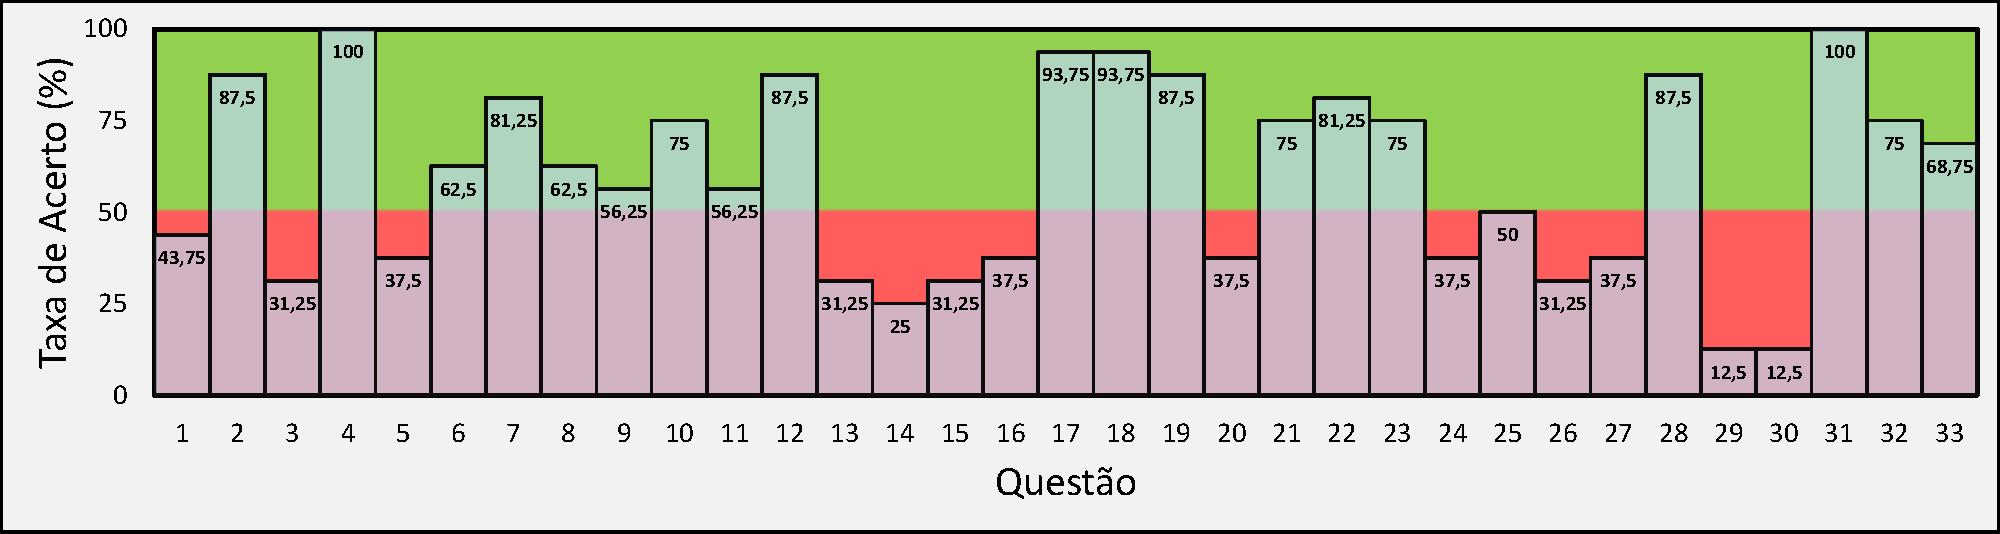
\includegraphics[width=\linewidth]{./Visuais/Notas4.pdf}
    \legend{Fonte: Elaborada pelo autor (2021).}
  
\end{figure}

A \autoref{fig:barrasCon} ilustra a taxa de acerto por questão (grupo controle). O eixo das abscissas representa cada uma das questões do questionário, sendo o número 1 (um) a primeira questão do questionário e o número 33 (trinta e três) a última questão do questionário. O eixo das ordenadas representa a taxa de acerto, indo de 0 (zero) a 100 (cem). O número 0 (zero) significa que nenhum indivíduo acertou aquela questão, o número 100 (cem) significa que aquela questão foi acertado por todos os indivíduos. No presente caso, tanto a questão 4 (quatro), quanto a questão 31 (trinta e um), tiveram uma taxa de acerto de 100\% para o grupo controle. O mesmo não ocorre com o grupo experimental como pode ser observado na \autoref{fig:barrasExp}.

\begin{figure}[htb]

    \caption{\label{fig:barrasExp}Gráfico de Barras da taxa de acerto por questão no pré-teste (grupo experimental).}
    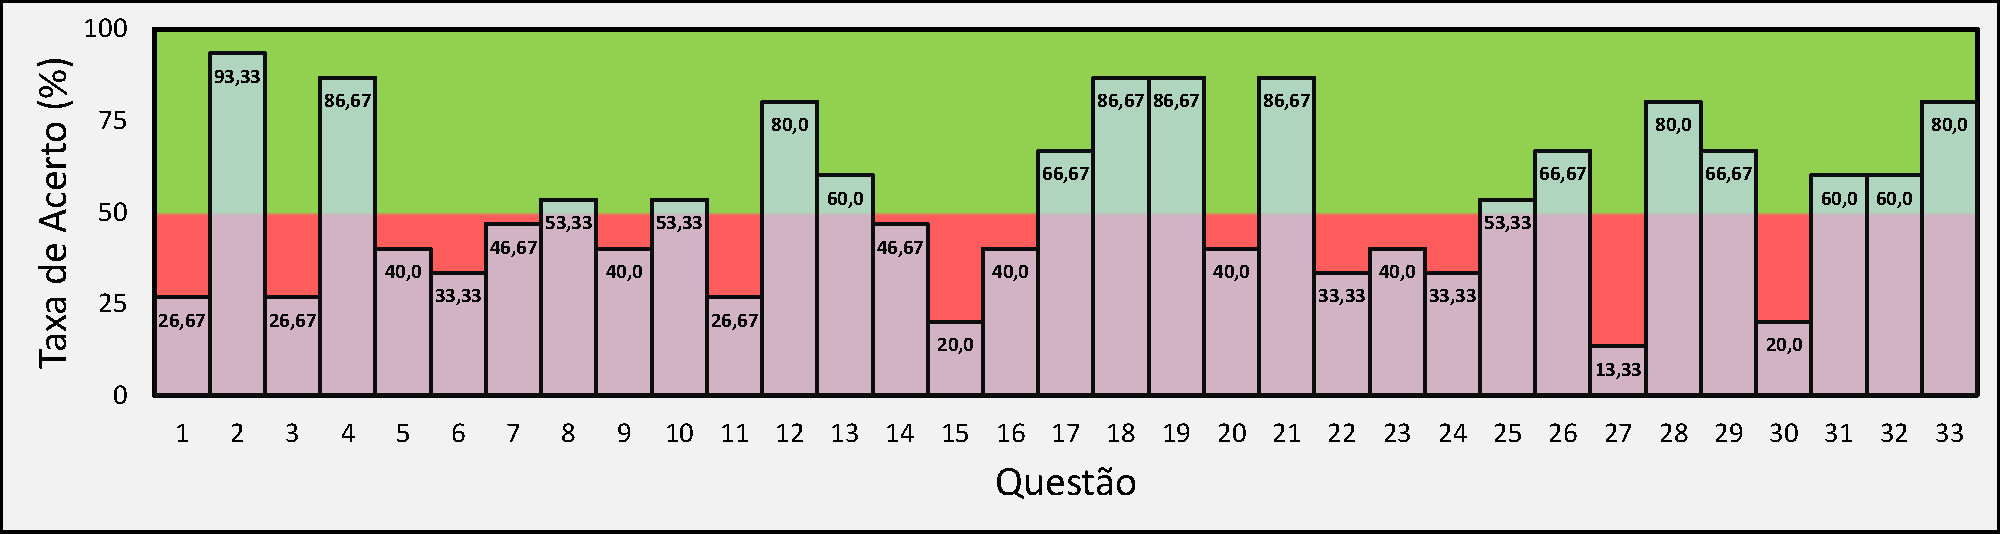
\includegraphics[width=\linewidth]{./Visuais/Notas3.pdf}
    \legend{Fonte: Elaborada pelo autor (2021).}
  
\end{figure}

A \autoref{fig:barrasExp} apresenta a taxa de acerto por questão (grupo experimental). Em comparação ao grupo controle (\autoref{fig:barrasCon}) o grupo experimental teve um desempenho ligeiramente inferior. Questões em branco ou rasuradas (de difícil identificação) foram consideradas erradas, ao total 26 (vinte e seis) questões estava rasuradas ou haviam sido deixadas em branco. Para fornecerem um panorama melhor da menor nota, maior nota e a média de cada grupo, produziu-se um diagrama de caixa estreita (\autoref{fig:caixapre}).


\begin{wrapfigure}[17]{r}{10.0cm}%pulando 17 linhas
    \vspace{-4pt}
    \caption{\label{fig:caixapre}Diagrama Caixa Estreita das notas (pré-teste).}
    \vspace{8pt}
    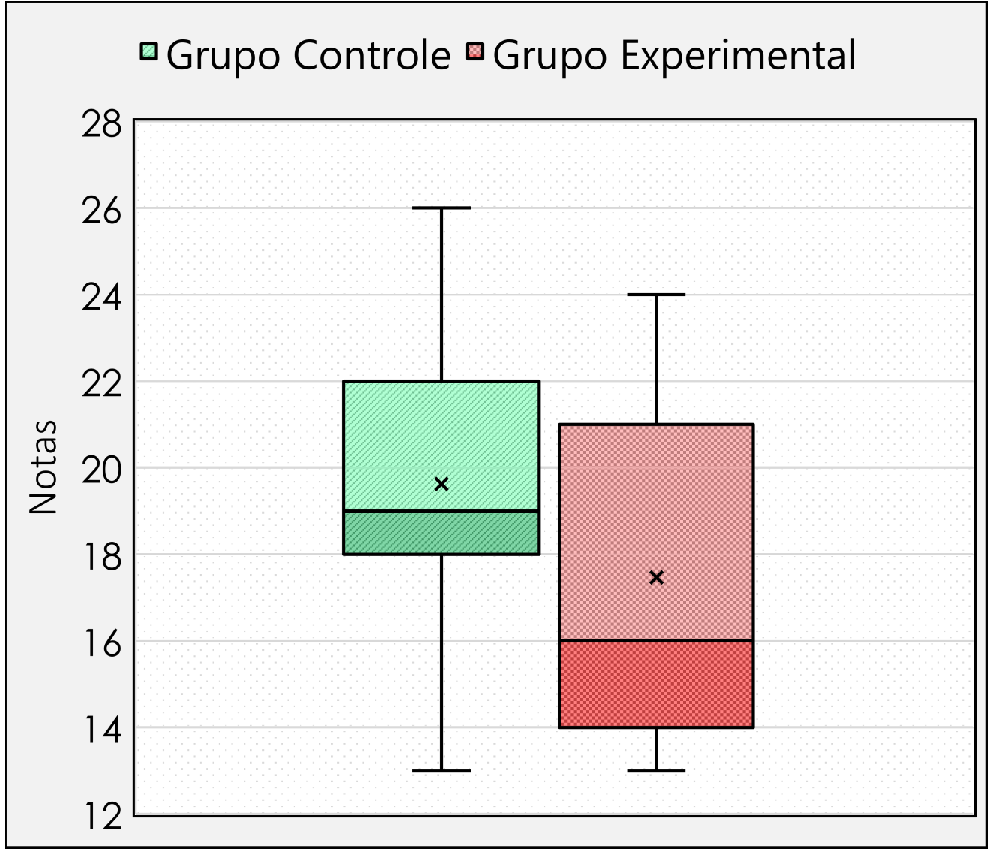
\includegraphics[width=\linewidth]{./Visuais/CaixaEstreitaEnfeitado.pdf}
    \legend{Fonte: Elaborada pelo autor (2021).}
\end{wrapfigure}

Um diagrama caixa estreita mostra a distribuição dos dados em quartis, realçando a média e as exceções. No caso do presente estudo o grupo controle acertou em média 19,625 ($\sigma$ = 3,18) questões (59,47\%, $\sigma$ = 9,64), enquanto o grupo experimental acertou em média 17,467 ($\sigma$ = 3,96) questões (52,93\%, $\sigma$ = 12), valores representados pela marcação em $\times$ na \autoref{fig:caixapre}. A maior quantidade de acertos foi de 26 (vinte e seis) questões no grupo controle e 24 (vinte e quatro) questões no grupo experimental. Ambos os grupos tiveram uma menor quantidade de acertos de 13 (treze) questões.

Para a devida condução da atual pesquisa é preciso garantir que as amostram sejam equivalentes entre si. Para averiguar o grau de equivalência entre duas amostras a estatística faz uso do Teste-T. Contudo, para se utilizar o Teste-T, é preciso determinar a priori, se a variância entre os grupos é igual ou diferente. Após os cálculos, os resultados indicaram que as  variâncias do grupo controle e grupo experimental são equivalentes ($\alpha$ = 0,05). Deste modo, o Teste-T foi realizado assumindo variância iguais entre as amostras, concluíndo ao final que as amostras são de fato, equivalentes ($\alpha$ = 0,05). A \autoref{fig:normal} ilustra a equivalência entre as amostras. 

\begin{figure}[htb]
    \centering
    \caption{\label{fig:normal}Distribuição das notas atingidas no pré-teste}
    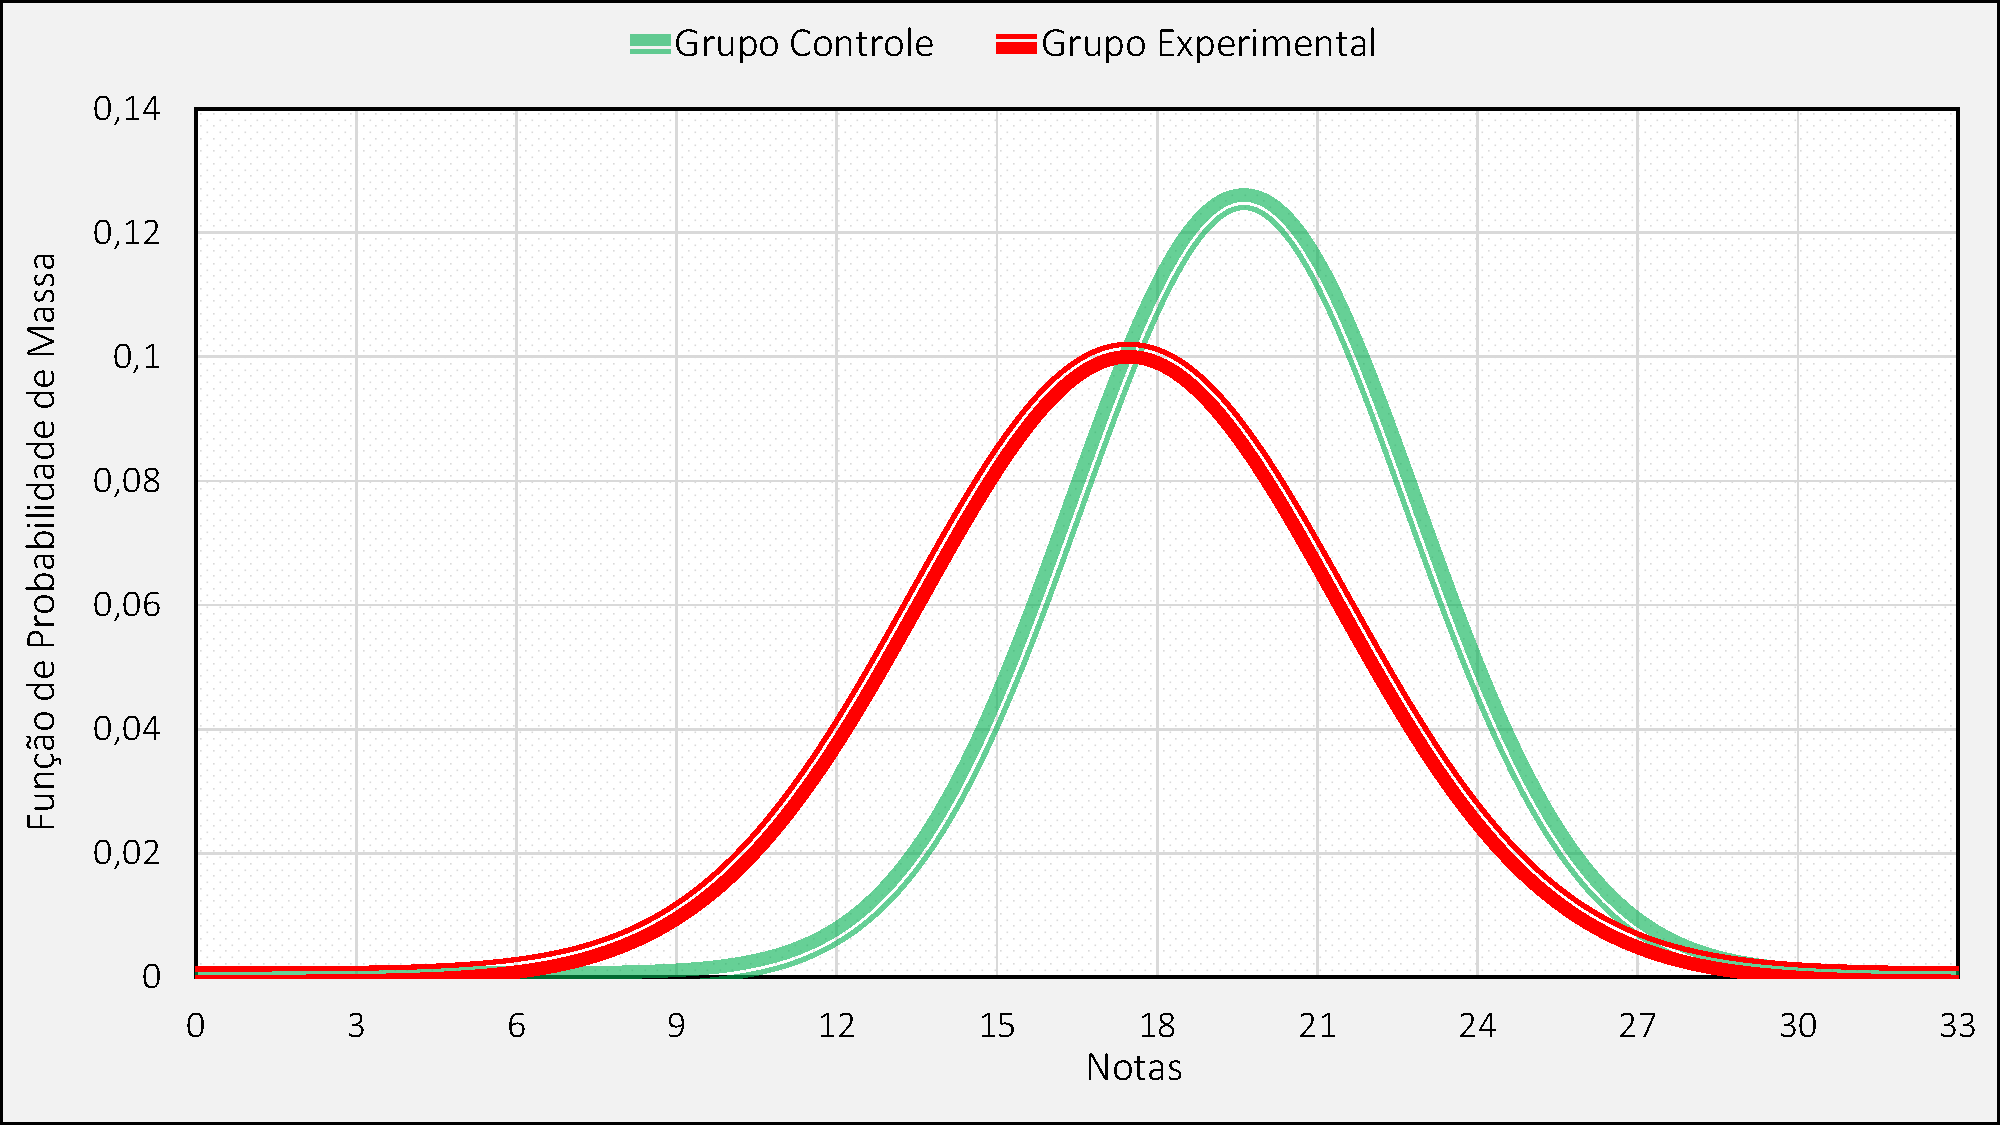
\includegraphics[width=\linewidth]{./Visuais/Graficos1.pdf}
    \legend{Fonte: Elaborada pelo autor (2021).}
  
\end{figure}


Para identificar se a variação dos dados refletiria em empecilhos para a presente pesquisa se realizou o Teste-F. Os resultados do Teste-F indicaram as variâncias entre o grupo controle e grupo experimental são iguais. Uma vez que sabia-se que as variância entre os grupo eram equivalentes se pode finalmente realizar o Teste-T para 

busca no geral, comparar duas amostrar, de modo a identificar se há diferenças significas entre elas ou não. 




\section{Teste}\label{sec:tes}

Praprado na escola 3 (três) de novembro de 2021 [Carla]

Primeiro dia na escola 4 (quatro) de novembro de 2021 [Carla]
 
Segundo dia na escola 5 (cinco) de novembro de 2021 [Rocilda]

\section{Pós-teste}\label{sec:postes}


Praprado na escola 25 (vinte e cinco) de novembro de 2021

\section{Apreciação}\label{sec:apreciar}

Praprado na escola 25 (vinte e cinco) de novembro de 2021

\section{Compilação}\label{sec:compilar}

\subsection{Meus}\label{subsec:meus}


112 crianças (Turmas C e D, 2 e 3)
2C = 8 crianças
2D = 12 crianças
3C = 10 crianças
3D = 3 crianças


\subsection{Comparativo}\label{subsec:outros}

%\section{Considerações Finais}\label{sec:compilar}


*Resultados Finais

*Conclusão







A atual pesquisa submente o instrumento avaliativo \ac{CKAQ} para sua amostra de participantes (grupo controle e grupo experimental). A submissão do \ac{CKAQ} ocorre em duas etapas distintas da presente pesquisa, inicialmente na etapa de pré-teste e posteriormente na etapa de pós-teste. O instrumento avaliativo é entregue de maneira impressa e administrado verbalmente em sala de aula e em horário escolar para todos os participantes válidos de uma turma. Participantes inválidos (\textit{e.g.} crianças com participação não aprovada por seus guardiões legais) são direcionados para um atividade escolar sob responsabilidade da escola. Após a administração do \ac{CKAQ}, suas cópias impressas com as respostas dos participantes são colhidas e embaralhadas. Tal coleta encerra a etapa de pré-teste e demarca o início da etapa de teste da presente pesquisa.

%Tal versão é submetida ao grupo controle e ao grupo experimental em momentos distintos de maneira coletiva. O questionário é adminitrado verbalmente e as crianças devem responde-lo em suas folhas. Cada criança tem um indetificador. O questionário tem previsão de ser respondido em 15 minutos. Essa etapa consiste em colher a Aprendizagem (dado quantitativo) sobre  a temática de ambos os grupos. O questionário pode ser administrado por um dos pesquisadores ou por outro responsável optado pela escola. Ao término do questionário as folhas serão colhidas de cada participantes para análise. 


%Os resultados alcançados com o grupo estudado se demonstrar bem sólidos e robustos. Isso pois, a presente pesquisa se utiliza do Teste-t com um grau de confiança de 95\%. A alta taxa de confiança estatística do presente estudo, abre margem para uma defesa sólida e robusta de seus resultados. 

TESTES TESTES.....

Uma turma com 112 (cento e doze crianças) foram seleciondas para participantarem dessa pesquisa da Escola Municipal Pauline Parucker. Todos os protoclos foram segufios....









